\documentclass[NewProceedings,letterpaper]{ascelike-new}
\WarningFilter{caption}{Unknown document class}
\usepackage[utf8]{inputenc}
\usepackage[T1]{fontenc}
\usepackage{graphicx}
\usepackage[style=base,figurename=Fig.,labelfont=bf,labelsep=period]{caption}
\usepackage{amsmath}
\usepackage{newtxtext,newtxmath}
\usepackage{booktabs}
\usepackage[table]{xcolor}
\usepackage{array}
\usepackage{microtype}
\usepackage{needspace}
\usepackage{placeins}
\usepackage{float}
\usepackage[hidelinks]{hyperref}
\definecolor{tableblue}{RGB}{228,240,249}
\hypersetup{pdftitle={Balancing Pedestrian Service and Robot Access: An Interpretable Admission Framework for Sidewalk Delivery Robots},pdfauthor={An Xu and Yunfei Yin}}
\captionsetup[figure]{skip=6pt}
\setlength{\belowcaptionskip}{4pt}
\pdfminorversion=7
\graphicspath{{figures/}}
% Generated from verified CICTP inputs.
\newcommand{\Candidates}{400}
\newcommand{\Cells}{140}
\newcommand{\MainScenarios}{280}
\newcommand{\AdditionalScenarios}{120}
\newcommand{\CorridorLength}{50}
\newcommand{\EngineVersion}{SUMO 1.27.1}
\newcommand{\PedRadius}{0.25}
\newcommand{\PedSpeed}{1.25}
\newcommand{\PedSD}{0.15}
\newcommand{\PedMin}{0.8}
\newcommand{\PedMax}{1.8}
\newcommand{\RobotLength}{0.96}
\newcommand{\RobotWidth}{0.7}
\newcommand{\RobotRadius}{0.48}
\newcommand{\RobotSpeed}{1.39}
\newcommand{\TimeStep}{0.1}
\newcommand{\Warmup}{100}
\newcommand{\Measurement}{240}
\newcommand{\Tail}{100}
\newcommand{\ZoneLength}{20}
\newcommand{\Timeout}{300}
\newcommand{\SpeedRetention}{0.90}
\newcommand{\DensityLimit}{1.20}
\newcommand{\FlowLow}{0.90}
\newcommand{\FlowHigh}{1.20}
\newcommand{\PassN}{29}
\newcommand{\SeedN}{30}
\newcommand{\QMax}{20}
\newcommand{\WidthMin}{1.6}
\newcommand{\WidthMax}{3.0}
\newcommand{\DemandMax}{60}
\newcommand{\SpecificMax}{\frac{100}{3}}
\newcommand{\SinuosityMax}{1.05}
\newcommand{\TurnAngle}{20}
\newcommand{\TurnRatio}{0.6}
\newcommand{\SpeedFloor}{0.8}
\newcommand{\MainC}{23.842}
\newcommand{\MainP}{-0.930}
\newcommand{\MZeroMargin}{3.376}
\newcommand{\EvalN}{164}
\newcommand{\EvalCells}{64}
\newcommand{\UtilN}{139}
\newcommand{\EvalCensored}{8}

\setlength{\textfloatsep}{11pt plus 2pt minus 2pt}
\setlength{\intextsep}{11pt plus 2pt minus 2pt}
\renewcommand{\topfraction}{0.9}
\renewcommand{\bottomfraction}{0.8}
\renewcommand{\textfraction}{0.08}
\renewcommand{\floatpagefraction}{0.90}
\makeatletter
\setlength{\@fptop}{0pt}
\setlength{\@fpbot}{0pt plus 1fil}
\makeatother
\NameTag{}
\begin{document}
\clubpenalty=10000 \widowpenalty=10000
\title{Balancing Pedestrian Service and Robot Access: An Interpretable Admission Framework for Sidewalk Delivery Robots}
\author[1]{An Xu}
\author[1,*]{Yunfei Yin}
\affil[1]{School of Transportation Science and Engineering,
Harbin Institute of Technology, Harbin 150090, China}
\affil[ ]{\texttt{AnX.RTL2324@tum-asia.edu.sg} (An Xu);
\texttt{yunfeiyin@hit.edu.cn} (Yunfei Yin)}
\maketitle
\begingroup
\renewcommand{\thefootnote}{*}
\footnotetext[0]{Corresponding author: Yunfei Yin (yunfeiyin@hit.edu.cn).}
\endgroup
\begin{abstract}
Sidewalk delivery robots offer a new option for urban logistics, but their access must be considered alongside pedestrian service. Operating permission and fleet size do not determine an appropriate entry rate for an individual sidewalk. This study develops an interpretable framework for that local allocation decision. The framework checks geometric applicability and pedestrian-only service, estimates a robot entry rate from width and pedestrian demand, and applies a conservative margin before direct service testing. Microscopic simulations use geometry--demand scenarios from seven cities, with coefficients and margins estimated through city-held-out evaluation. Across five margin settings, greater conservativeness reduces observed service failures while withholding more robot access. The original conservative setting admits robots in 98 scenarios with no observed failures, compared with 136 scenarios and 18 failures without a margin. Many withheld opportunities nevertheless pass at their directly tested rates. Stratified independent-seed tests support the stability of the conservative recommendations in the selected cases. Transfer to irregular sidewalk polygons and changes in robot size and pedestrian direction show that local configuration also matters. The framework makes the access--service trade-off explicit and supports assessment under stated operating conditions.
\end{abstract}
\KeyWords{sidewalk delivery robots; pedestrian service; admission control; microscopic simulation; urban logistics}

\section{Introduction}
Sidewalk delivery robots are being explored for parcel and grocery delivery over the final part of an urban trip. Their potential benefits have motivated studies of freight efficiency and last-mile operations \cite{Jennings2019,Alverhed2024}. These robots also use space that is primarily intended for walking (Fig.~\ref{fig:scene}). As deployment expands, managing the amount of robot traffic becomes a pedestrian-service question as well as a logistics question.

\begin{figure}[!htbp]
\centering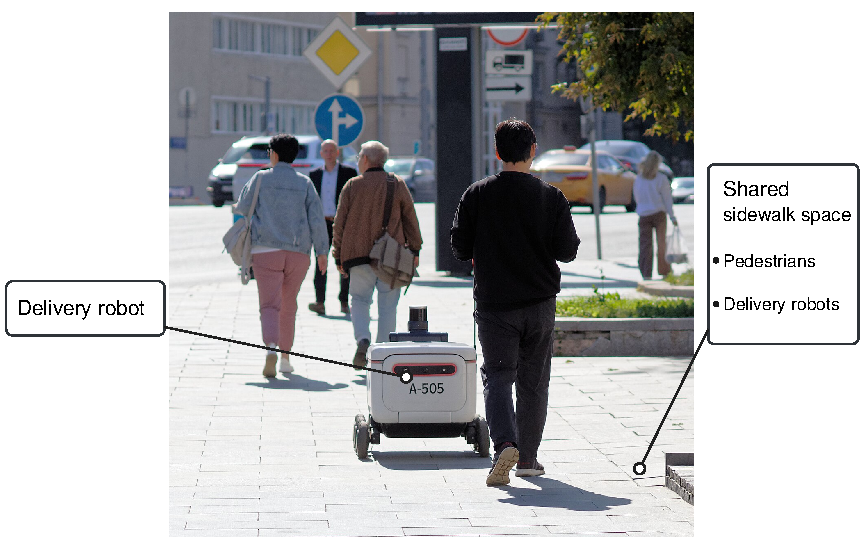
\includegraphics[width=\textwidth]{visual_revision_20261008/figures/figure1_scene.pdf}
\caption{Illustrative sidewalk-delivery-robot scene in an urban pedestrian environment. The image motivates the local admission problem studied in this paper: how much robot access should be offered while acceptable pedestrian service is maintained. Photograph: Retired electrician / \href{https://commons.wikimedia.org/wiki/File:Moscow,_Yandex_employee_walking_his_pet_A-505_robot,_Aug_2025_04.jpg}{Wikimedia Commons}, \href{https://creativecommons.org/publicdomain/zero/1.0/}{CC0 1.0}; vector annotations added by the authors.}
\label{fig:scene}
\end{figure}

Operating permissions and fleet allowances govern deployment at a broader scale \cite{Kovacica2024,DDOTPDD}. They do not specify how many robots should enter a particular sidewalk during a period of pedestrian activity. The same fleet can impose different local loads depending on route concentration and demand. Sidewalk width provides space for encounters and passing, while pedestrian demand determines how intensively that space is used. Local entry-rate management therefore requires more information than a permit or fleet total.

Quantitative interaction studies measure different aspects of shared-space performance. Corridor experiments show that a crossing mobile robot can reduce collective pedestrian speed \cite{Chen2018}. Laboratory-calibrated simulations evaluate a person-following delivery robot's speed under changing crowd density, direction and corridor width \cite{Li2025}. Field studies examine encounter conflicts and pedestrian or cyclist responses \cite{Gehrke2022}, while routing models account for uncertain sidewalk travel conditions \cite{TongSimoni2026}. These studies inform interaction and deployment assessment. The present study instead treats robot entry flow as the allocation variable and tests each offered rate against a stated pedestrian-service objective.

A flow estimate alone is insufficient for that local decision. It may apply outside its assessed geometric range, or it may offer access where the pedestrian-only condition already performs poorly. Even under suitable conditions, a conservative rate can protect service at the cost of useful delivery access.

This study addresses that allocation problem through an interpretable admission framework. Local checks determine whether assessment is appropriate, and a width--demand relation proposes a candidate entry rate. A controllable margin reduces that rate before its service performance is tested directly. The contributions are a clear local admission procedure, evidence of how conservativeness changes both access and pedestrian service, and an assessment of the role of geometry and operating conditions. By varying the margin under a common service objective, the study examines how much access is withheld to reduce service deterioration.

\section{Methodology}
\subsection{Sidewalk Scenarios and Simulation}
The development sample contains \Candidates{} geometry--demand scenarios from \Cells{} sidewalk cells in Amsterdam, Melbourne, New Taipei, New York, Seattle, Taipei, and Taoyuan. GIS-derived widths and centreline descriptors define idealized corridors of nominal length \CorridorLength{}~m. The \MainScenarios{} main scenarios use pedestrian-demand priors informed by nearby residential, commercial, tourism, and transit activity. Another \AdditionalScenarios{} scenarios extend the demand range. These are controlled experimental inputs, not observed pedestrian arrivals in the seven cities.

Simulations use \EngineVersion{} with JuPedSim \cite{Lopez2018}. Both agent types use its collision-free-speed implementation, with robots represented by a larger walking-agent type. Pedestrians have radius \PedRadius{}~m and desired speeds with mean \PedSpeed{}~m/s and standard deviation \PedSD{}~m/s, bounded by \PedMin{} and \PedMax{}~m/s. The reference robot has dimensions \RobotLength{} by \RobotWidth{}~m and nominal speed \RobotSpeed{}~m/s. Its interaction representation is a collision disc of radius \RobotRadius{}~m. Pedestrians travel equally in both directions, while robots enter in one direction. Regular arrival schedules specify demand, and random seeds vary stochastic agent properties.

Each run uses a \TimeStep{}~s time step, a \Warmup{}~s warm-up and a \Measurement{}~s measurement window, followed by a \Tail{}~s completion period. Speed and density are measured in a central \ZoneLength{}~m zone. For irregular polygons, positions are projected onto the measurement axis; zone length times representative width supplies the density denominator. Polygon erosion by the robot radius checks geometric feasibility before evaluation. Cases without a feasible robot-centre region, or without completed measurements because of the \Timeout{}~s runtime limit, are excluded. Completed adverse outcomes remain in the analysis.

\subsection{Pedestrian Service and the Reference Flow}
The service objective combines walking speed, pedestrian density and completed-trip balance. For seed $s$, $\bar v_s$ is mean pedestrian speed in the measurement zone and window, and $\bar k_s$ is the mean zone count divided by its area. Robots are excluded from both measures. Baseline speed $v_0$ is the mean of the 30 pedestrian-only seed means for the same configuration. A seed qualifies when
\begin{equation}
 \bar v_s/v_0\geq\SpeedRetention{},\qquad
 \bar k_s\leq\DensityLimit{},\qquad
 \FlowLow{}\leq T_s\leq\FlowHigh{}.
 \label{eq:service}
\end{equation}
Density is measured in ped/m$^2$. The flow ratio $T_s=N_{\rm arr,s}^{\rm comp}/N_{\rm dep,s}^{\rm comp}$ compares completed records arriving and departing during measurement. A zero denominator is undefined and fails the flow component. This ratio measures balance among completed records, not fulfillment of all scheduled demand. Scheduled demand, first observations and completed trips are therefore checked separately; first observation is not a physical insertion timestamp.

A tested flow passes when at least \PassN{} of \SeedN{} seeds satisfy Eq.~\ref{eq:service}. The same acceptance rule evaluates the pedestrian-only baseline, with $B=1$ denoting qualification. Conditional on a qualifying baseline, the reference $q^*$ is the highest qualifying robot flow in the original finite scan. Discrete coarse tests cover 0--10~robots/min; selective higher-flow tests and integer refinements extend the scan up to \QMax{}~robots/min. The reference is zero when no positive scanned flow qualifies and is ceiling-censored at \QMax{}~robots/min. Unsupported and technically unresolved references remain undefined. The complete scan support is provided in the research repository.

\begin{figure}[H]
\centering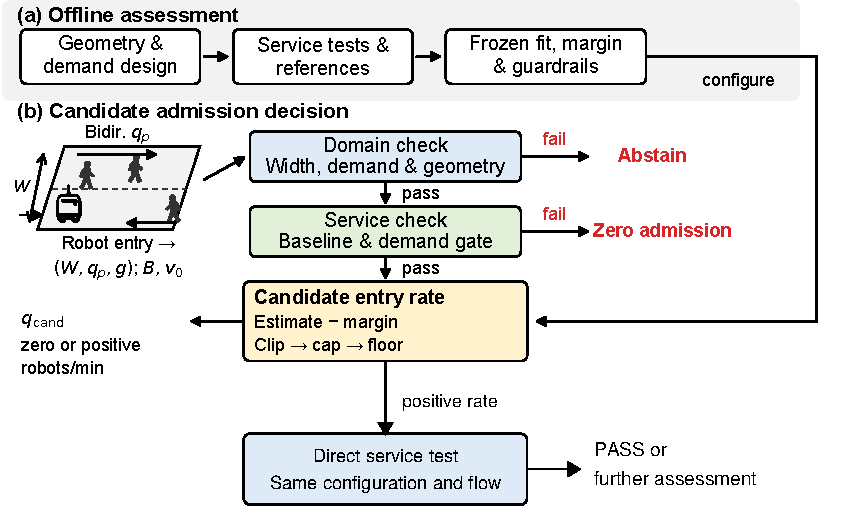
\includegraphics[width=\textwidth]{visual_revision_20261008/figures/figure2_framework.pdf}
\caption{Local robot admission. Geometry and pedestrian-service checks precede the candidate entry rate. A positive rate receives a configuration-matched service test.}
\label{fig:framework}
\end{figure}

\subsection{Admission Checks and Conservative Allocation}
Figure~\ref{fig:framework} distinguishes an unsupported condition, zero admission and a positive candidate rate. The applicability domain $\mathcal D$ covers widths of \WidthMin{}--\WidthMax{}~m and positive pedestrian demand up to \DemandMax{}~ped/min. Specific demand is $x=q_p/W<\SpecificMax{}$~ped/(min\,m). Straight corridors and mildly curved corridors with sinuosity no greater than \SinuosityMax{} are assessed. Concentrated turns are excluded when maximum and cumulative angles both reach \TurnAngle{} degrees and their ratio reaches \TurnRatio{}.

Within the domain, the service gate $G$ requires a qualifying pedestrian baseline, $v_0\geq\SpeedFloor{}$~m/s and $q_p<C(W)$. The nominal width--demand estimate is
\begin{equation}
 q_{\rm nom}=cW(q_p/W)^p,\qquad
 \log(q^*/W)=\log c+p\log x+\varepsilon.
 \label{eq:nominal}
\end{equation}
Ordinary least squares uses positive uncensored training references. An additive margin $\Delta$ is the selected linearly interpolated empirical quantile of $[q_{\rm nom}-q^*]_+$ over all training cases with defined references, including zeros and ceiling-censored observations. Fitting and margin calibration retain the recorded rounded $x$ values; prediction evaluates $q_p/W$ from the stored inputs.

For valid inputs within $\mathcal D$, define the bounded rate $q_b$. The offered integer entry rate is
\begin{equation}
\begin{aligned}
q_b&=\min\{q_{\max},Q_{\rm low}(W),[q_{\rm nom}-\Delta]_+\},\\[2pt]
q_{\rm cand}&=\begin{cases}
\text{abstain},&\text{invalid inputs or outside }\mathcal D,\\
0,&\text{within }\mathcal D,\ G=0,\\
\lfloor q_b\rfloor,&\text{within }\mathcal D,\ G=1.
\end{cases}
\end{aligned}
\label{eq:quota}
\end{equation}
Here $[z]_+=\max(0,z)$, $g$ describes geometry and $q_{\max}=\QMax{}$~robots/min. The demand gate and low-demand ceiling are fixed guardrails developed from synthetic width--demand experiments. Table~\ref{tab:guards} supplies their values, with linear interpolation between widths. Margin subtraction can produce zero even when the service gate passes. At fixed specific demand, Eq.~\ref{eq:nominal} scales linearly with width; its full-development exponent $p=\MainP{}$ implies approximately $W^{1.93}q_p^{-0.93}$. This is an empirical scaling relation over the assessed domain.

\begin{table}[!htbp]
\centering\caption{Demand gate and flow ceiling at assessed widths.}
\label{tab:guards}\setlength{\tabcolsep}{4.4pt}
\begin{tabular}{lrrrrrrr}
\toprule
$W$ (m) & 1.6 & 1.7 & 1.8 & 2.1 & 2.4 & 2.7 & 3 \\
\midrule
$C(W)$ (ped/min) & 35 & 35 & 45 & 45 & 55 & 90 & 90 \\
$Q_{\rm low}(W)$ (robots/min) & 5 & 6 & 8 & 10 & 18 & 20 & 20 \\
\bottomrule
\end{tabular}

\end{table}

\subsection{Evaluation Design}
Four allocation rules use the same applicability checks and ceilings. M0 applies the width--demand estimator with a 0.80-quantile margin; M1 removes that margin. M2 uses a width-only relation, $\log q_{\rm nom}=a+b\log W$. M3 estimates free width and demand exponents, $\log q_{\rm nom}=a+b\log W+d\log q_p$. M2 and M3 have their own 0.80-quantile margins. In contrast, M0 imposes $b+d=1$ and estimates two coefficients.

In each city-held-out fold, coefficients and margins are estimated on six cities and applied to the seventh. Applicability rules, demand gates and ceilings remain fixed development choices, including rules informed by earlier city-geometry diagnostics. Thus, the folds assess coefficient and margin transfer under an already developed admission structure. Screening leaves \EvalN{} evaluated scenarios from \EvalCells{} cells. The comparison also tests margin quantiles 0.50, 0.65, 0.80 and 0.90, alongside a no-margin condition with $\Delta=0$. These settings were specified before the extension tests and were not selected using held-out service outcomes.

Every positive recommendation is tested at its exact scenario, entrance configuration, integer flow and seed block. Coinciding recommendations share the same evidence rather than count as independent corroboration \cite{jin2026agreement}. Primary tests use seeds 0--29 and their matching baseline. PASS and FAIL partition positive recommendations; zero admission is not a service pass. Service at a candidate below $q^*$ is tested directly rather than inferred from that reference.

Independent replication uses seeds 10000--10029 and matching pedestrian-only baselines. Fifteen scenarios were selected deterministically from the original seed results and frozen before these runs. They comprise five robust M0 cases with 30/30 qualifying seeds and larger threshold clearance, five near-boundary M0 cases with 29/30, and five M1-failure cases spanning failure severity. Two M0 recommendations are zero, leaving 13 positive M0 conditions and 15 positive M1 conditions. Candidate rates remain unchanged. Robot access is summarized by the number of positive recommendations and the offered flow; pedestrian service is assessed at those rates. Median reference utilization is
\begin{equation}
 U=\operatorname{median}_{i:q_i^*>0}(q_{{\rm cand},i}/q_i^*).
 \label{eq:utilization}
\end{equation}
It includes zero recommendations among \UtilN{} positive-reference scenarios and does not clip ratios above one. The denominator also includes \EvalCensored{} ceiling-censored references.

Hong Kong transfer applies the full-development parameters $c=\MainC{}$, $p=\MainP{}$ and M0 margin $\Delta=\MZeroMargin{}$~robots/min without refitting. Thirteen final configurations retain their original entrances, and five use geometry-based entrance repairs within unchanged polygons. Each configuration has a separate baseline. Operating-condition tests use two width-order-selected scenarios at 4~robots/min. They vary robot size and the share of pedestrians traveling against the robots, with a matching baseline for each setting.

\section{Results}
\subsection{Conservativeness Changes Both Service and Access}
The margin sweep shows that reducing failed service tests requires giving up some robot access (Fig.~\ref{fig:tradeoff}). Without a margin, 136 scenarios receive positive rates and 18 fail. At the M0 quantile of 0.80, all 98 positive recommendations pass. A further increase to 0.90 leaves 58 positive recommendations, also with no observed failures. The intermediate settings show how the margin can adjust the balance between these outcomes. The 0.80 setting retains more opportunities than 0.90 at the same observed failure count in this sample; it is not a universal optimum.

\begin{figure}[!htbp]
\centering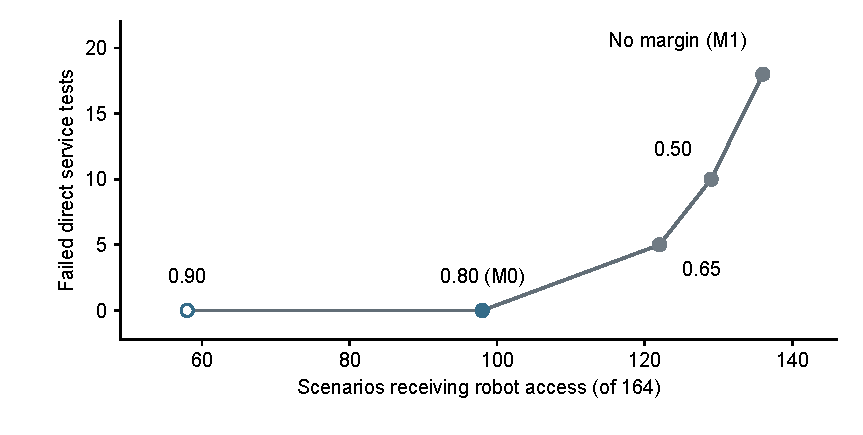
\includegraphics[width=\textwidth]{visual_revision_20261008/figures/figure3_tradeoff.pdf}
\caption{Observed access--service trade-off across five prespecified margin settings. Each point combines positive recommendations and failed direct tests on the 164 evaluated scenarios. The connecting line indicates the tested sequence, not an interpolated service guarantee.}
\label{fig:tradeoff}
\end{figure}

Conservativeness changes both where robots receive access and the rates offered there. Among the 98 scenarios admitted by M0 and M1, the mean rate decreases from 7.55 to 4.81~robots/min. M1 fails in 12 of these cases, whereas M0 passes in all 98. M0 also withholds 38 opportunities offered by M1, of which 32 pass at their directly tested zero-margin rates. These passing opportunities show the cost of a margin that is applied before local service evidence is available.

Table~\ref{tab:methods} places the margin comparison alongside the alternative estimators. Relaxing the width--demand scaling constraint in M3 retains the same number of positive recommendations as M0 but introduces two failures. The width-only rule offers fewer opportunities. These are comparisons of complete allocation rules because each alternative calibrates its own margin. In this evaluated sample, the choice of conservativeness changes access and service more substantially than the M0--M3 change in estimator form.

\begin{table}[!htbp]
\centering\caption{Core allocation rules on 164 scenarios. Utilization uses all 139 positive-reference scenarios, including zero admission.}
\label{tab:methods}\small\setlength{\tabcolsep}{6pt}
\begin{tabular}{lrrrrr}
\toprule
Rule & Positive & Zero & PASS & FAIL & $U$ (\%) \\
\midrule
\rowcolor{tableblue}
M0: width--demand + margin & 98 & 66 & 98 & 0 & 16.7 \\
M1: no margin & 136 & 28 & 118 & 18 & 75.0 \\
M2: width only & 59 & 105 & 59 & 0 & 0.0 \\
M3: free exponents & 98 & 66 & 96 & 2 & 18.2 \\
\bottomrule
\end{tabular}

\end{table}

\subsection{Walking Speed Is a Major Service Constraint}
Pedestrian speed is involved in all 18 original zero-margin failure groups and is the dominant failed component in 17. Ten groups have speed failures without density or flow-ratio failures. The speed criterion can therefore identify deterioration even when average zone density stays within its limit. Component labels combine the evidence across seeds within each scenario, rather than implying simultaneous failures in every run.

The median of the group-median speed-retention values is 0.982 for M0 and 0.963 for M1. This difference is consistent with the more conservative rates placing less pressure on walking service. Supporting demand checks find no original M0 seed with completed-window arrivals below 90\% of scheduled-window demand. Occasional qualifying comparator seeds have larger shortfalls, which are documented in the repository alongside the separate demand diagnostics.

\subsection{Boundary Decisions Are Sensitive to Stochastic Realization}
Independent seeds preserve all 13 replicated positive M0 decisions, while only 7 of 15 M1 decisions remain unchanged. M1 transitions occur in both directions: two passes become failures and six failures become passes. Both methods are stable in the robust stratum, whereas changes occur in the boundary and failure strata. The deliberately stratified sample supports the stability of the tested conservative recommendations and identifies sensitivity near the service boundary. It does not estimate reliability across the full scenario population.

\subsection{Geometry and Operating Conditions Affect Admission}
The Hong Kong results show that entrance configuration influences whether a sidewalk can be assessed (Fig.~\ref{fig:hk}). Original entrances support 13 configurations; geometry-based repairs make another five sites evaluable. M0 offers seven positive rates in the original group and four in the repaired group, all passing. M1 offers 11 and five positives, with one failure among the original configurations. More offered access thus remains associated with a service trade-off after transfer. The extra evaluable sites do not constitute a before--after service comparison at identical entrances. Figure~\ref{fig:hk} shows eight examples selected by geometry and entrance-repair characteristics; the reported totals use all 18 configurations.

\begin{figure}[H]
\centering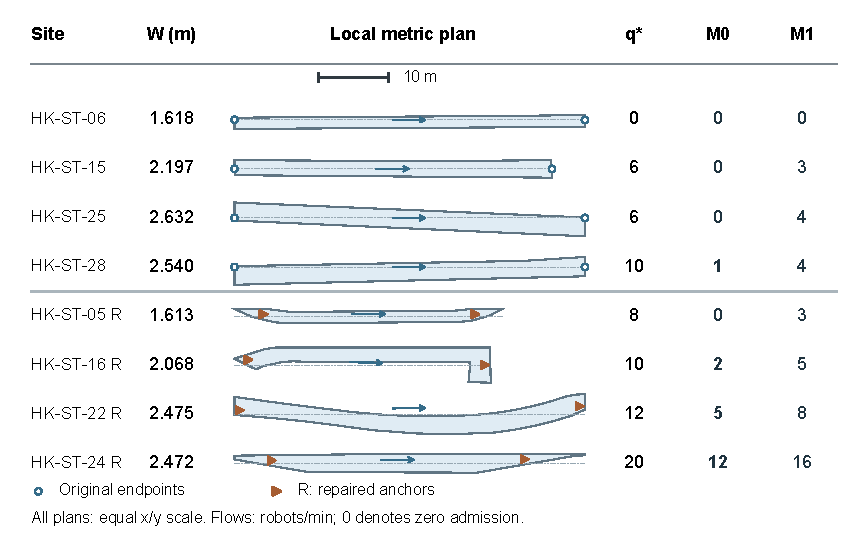
\includegraphics[width=\textwidth]{visual_revision_20261008/figures/figure4_hk_representative.pdf}
\caption{Eight geometrically selected Hong Kong configurations at a common metric scale. Each polygon retains its recorded local orientation and equal longitudinal and transverse scales. $W$ is the representative input width. Circles mark original centreline endpoints; triangles mark repaired entrance anchors (R). Arrows indicate robot direction. Reference and M0/M1 candidate flows are in robots/min. Zero admission is not a service pass. The \href{https://github.com/AnXu-ITS/sidewalk-robot-quota/blob/main/paper_CICTP2027/figures/hong_kong_all18_metric.pdf}{complete 18-configuration figure} and selection rule are available in the repository.}
\label{fig:hk}
\end{figure}

Operating assumptions can change service at the same entry rate (Table~\ref{tab:sensitivity}). Increasing the robot interaction radius from 0.480 to 0.575~m changes the narrow case from 30/30 to 0/30 passing seeds, while the wider case remains at 30/30. Increasing opposing pedestrian flow also lowers the passing-seed counts. These cases illustrate why a rate assessed for one robot body or directional composition requires renewed service assessment when those conditions change.

\begin{table}[!htbp]
\centering\caption{Operating-condition tests at 4~robots/min. Passing seeds are out of 30; each setting has its own baseline. Narrow: $W=1.75$~m, $q_p=21$~ped/min. Wide: $W=2.4$~m, $q_p=43.2$~ped/min. Radii are those used in the simulations.}
\label{tab:sensitivity}\small\setlength{\tabcolsep}{8pt}
\begin{tabular}{rrrr}
\toprule
Robot radius (m) & Opposing pedestrians (\%) & Narrow & Wide \\
\midrule
0.385 & 50 & 30 & 30 \\
0.480 & 50 & 30 & 30 \\
0.575 & 50 & \cellcolor{tableblue}0 & 30 \\
0.480 & 75 & 28 & 29 \\
\bottomrule
\end{tabular}

\end{table}

\FloatBarrier
\Needspace{6\baselineskip}
\section{Discussion}
Conservative admission is a management choice about the balance between delivery access and walking service. A margin can reduce the rate offered on an admitted sidewalk and can withhold access altogether. Its value should therefore be judged alongside the opportunities it removes, rather than by regression error alone. The passing zero-margin opportunities withheld by M0 make this distinction concrete. The useful decision is how much conservativeness is appropriate for the stated service objective and operating conditions.

Width provides room for movement, but that space does not translate into unrestricted robot flow. Pedestrian demand, opposing movement and robot size change how the available width is used. Entrance configuration further determines whether a geometric input produces a meaningful service assessment. These findings connect allocation to local traffic conditions: a fleet allowance cannot substitute for a segment-specific assessment, and a wider corridor can still require a restricted entry rate.

The framework supplies a candidate rate that can be assessed with direct service evidence. This offers an interpretable way to compare deployment choices while keeping the assumptions behind each recommendation visible. It is an offline assessment procedure rather than a feedback controller. An operational application would also need measured pedestrian demand and a calibrated representation of robot interactions.

The findings are bounded by circular robot interaction discs without a separately calibrated yielding controller, regular arrival schedules and finite stochastic tests. The service objective concerns walking conditions rather than collision safety. Hong Kong provides simulation geometry transfer, not field validation, and the assessed domain remains restricted. Field observations and tests of variable demand would be needed to determine how the procedure performs under changing sidewalk use.

\section{Conclusion}
Sidewalk robot admission can be treated as a local allocation decision that makes the trade-off between pedestrian service and delivery access visible. The proposed framework combines applicability checks, a width--demand estimate and a controllable margin, then tests each positive rate directly. In the evaluated sample, the original conservative setting reduces failed recommendations from 18 to zero while reducing positive access from 136 to 98. Some withheld opportunities nevertheless pass their direct tests, so greater conservativeness also has an access cost. Geometry and operating-condition evidence supports pairing each recommendation with its stated local conditions. The framework provides a basis for service-aware sidewalk assessment without assigning a universal robot capacity.

\section*{Data Availability}
Scenario data, simulation configurations, reproduction scripts and detailed experimental results are available in the versioned \href{https://github.com/AnXu-ITS/sidewalk-robot-quota/releases/tag/cictp2027-v1.0.0}{CICTP 2027 v1.0.0 research release}.

\section*{Acknowledgments}
This work was supported in part by the National Natural Science Foundation of China (Nos. 62673168 and 62303134) and the Fundamental Research Funds for the Central Universities (No. XNJKKGYDJ2024012).

\Needspace{5\baselineskip}
\bibliography{ascexmpl-new}
\end{document}
